\documentclass{article}
\usepackage[utf8]{inputenc}
\usepackage{graphicx}
\usepackage{lscape}
\usepackage{natbib}
\usepackage{hyperref}
\usepackage{rotating}
\usepackage{svg}
\usepackage{mathabx}

\usepackage{xcolor}
\usepackage{listings}
\lstset{basicstyle=\ttfamily,
  showstringspaces=false,
  commentstyle=\color{red},
  keywordstyle=\color{blue}
}
\usepackage{subfiles}

\usepackage{geometry}

\title{Software Maintenance and Evolution \\God Components}
\author{Jeroen G S Overschie (s2995697)\\ Konstantina Gkikopouli (s3751309)}
\date{\today}

\begin{document}
\maketitle
Repository: \small{\url{https://github.com/dunnkers/sme_god-components}}
\tableofcontents
\newpage

\section{Introduction}
God Components (or 'God objects') are components in a software system that have accumulated a large bulk of classes and lines of code over time. Such really large, bulky components are hard to maintain and to reason about; they are in fact a software \textit{anti-pattern} \citep{smith2000software}. It is preferred to have smaller, isolated components instead. Although it is a common good practice to build software by creating small building blocks of reusable code and accessing them using a declarative and well-documented API, big code-bases might still suffer from scaling issues: large inter-weaved software components might develop that become difficult to reason about.

To prevent God Components in your software, it is at all times important to keep refactoring a code-base at the architecture level, i.e. apply step-wise evolution \citep{toward_a_catalogue_of_architetural_bad_smells}. Be wary and suspicious about 'vague' abstractions that seem to want to answer too many questions at once \citep{riel1996object}. God Components might be broken up into separate, independent components that each have their separate function. This makes the code easier to test and reason about - and above all; more understandable to the humans actually maintaining the code-base.

In this project, one such analysis will be ran on the \textbf{Apache Tika} project \citep{apache_software_foundation_2020}. Apache Tika is a software package built to detect and extract text and metadata from many different file formats. File formats include PDF, PPT and XLS, and can all be accessed through Tika's API, making it easy to process a large amount of files using just a concise amount of code. Besides its text extraction capabilities, it is also commonly used to classify documents using meta-data obtain from Tika, such as any file's extension \citep{Tika}.

God Components will not only be identified, but their evolution over time will also be tracked. This will be done by searching for commits associated to one such God Component and observing either growth or shrinkage.

\section{Exploration}
First, we explore our chosen software project, Apache Tika, by means of \textbf{requirements analysis}. \citep{dresner1964maintenance}. Requirements were compiled using the project's public website \citep{apache_software_foundation_2020} and an online book about Apache Tika written by the authors \citep{tika_in_action}. 
\subsection{Tika's High-Level Architecture}
This section focuses on describing and explaining the high-level architecture of Tika. All the architecture’s components and their interactions are visualized in the simple diagram, i.e. Figure~\ref{fig:architectur}.
\subsubsection{Tika's Architecture}
The high-level architecture of Tika consists of four key components: the parser framework, the language detection, the MIME detection mechanism and the facade element. All these components play an important role in Tika’s overall architecture and they have their own corresponding responsibilities and functionalities. Firstly, the parser framework is the most crucial concept and its main functionality is parsing and extracting all the content and the relevant metadata of any type of document. The language detection component is responsible for carrying out language analysis and this helps in obtaining the metadata of the files. In addition, the MIME detection mechanism is used for detecting and identifying all the available file formats. All these three components contain their own individual repositories, which help in extending Tika by adding or removing new parsers, file formats or language mechanisms. Moreover, Tika’s architecture contains a facade, which connects all the main components and it provides a user-friendly frontend for the users that want to benefit from Tika’s services. The architecture also consists of some external interfaces like the CLI and the GUI, which allow integrability between users and their applications.

\begin{figure}[ht]
    \centering
    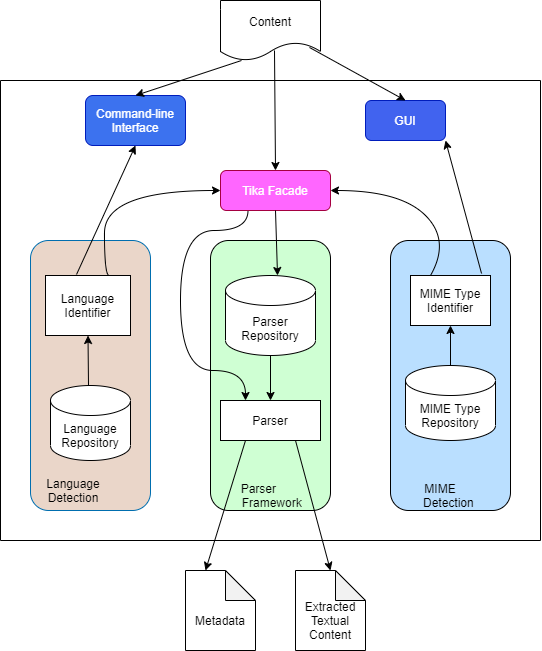
\includegraphics[width=0.85\textwidth]{report/images/tika_architecture.png}
    \caption{High-Level Architecture. Image composed by ourselves.}
    \label{fig:architectur}
\end{figure}

\subsection{Key design goals}
Let us denote the most important goals the authors set out to accomplish in creating Apache Tika.
\subsubsection{Unified parsing}
One of the initial key goals set by the creators of Apache Tika was the implementation of a unified parsing interface \citep{tika_in_action}.  In Apache Tika, unified parsing offers a collection of functionalities and a Java interface that deal with external third-party parsing libraries. This was achieved by the creation of the org.apache.tika.parser.Parser interface, which parses the received content incrementally.

\subsubsection{Low Memory Footprint and Fast Processing}
The second goal of the authors regarding Apache Tika was to achieve a low memory footprint and guarantee a fast processing performance \citep{tika_in_action}. The creators wanted to make sure that Tika could be easily integrated into any Java application at a low memory cost. This would be beneficial to the users, as they could run Tika in any environment ranging from mobile PDA to desktop computers. At the same time, Tika is expected to react quickly to user’s requests and perform file format identification and processing in a fast manner.

As mentioned previously, the received content is parsed incrementally and it is generated as SAX-based XHTML events. SAX (Simple API for XML processing) was the main XML parsing option, as it accomplished all the requirements regarding low memory footprint, fast processing and incremental parsing. In addition, SAX model is more flexible, as it allows its users to decide themselves on how they want to deal with the received content by modifying Tika’s parser and specifying what needs to be done atorg.xml.sax.ContentHandlers.

\subsubsection{Flexible Metadata}
Another design consideration was to ensure the required flexibility that Tika needs in order to perform its tasks on the extracted content \citep{tika_in_action}. There is an enormous amount of available file formats and Tika is capable of understanding and processing all of them. However, most of these formats contain associated metadata models that provide detailed descriptions about these files. In this case, Tika should also be able to understand the corresponding metadata models. In the previous releases, Tika was always modifying and generalizing the metadata of the extracted content, so that it could fit to its predefined structure. In the latest releases, Tika is not following the same technique and it has become more flexible, as it stores the metadata in their original form.

\subsubsection{Parser integration}
Another key design goal that was taken into account was the parser integration \citep{tika_in_action}. Similar to the metadata models and file formats, there are also a lot of parsing libraries and Tika has to easily integrate them within the application. According to the creators, from a design perspective Tika virtualizes the underlying parser libraries and ensures their conformance to Tika’s parser interface. However, this is a complicated task as the authors had to deal with parser exceptions, threads of control, delegation, and nuances in each of these libraries. Even though it was a cost-effective process, it brought a lot of benefits like cross-document comparison, uniformity, standardized metadata and extracted text.

\subsubsection{MIME Database}
Another design consideration was focused on the usage of MIME database, which contains a simple and an efficient way of categorizing the file formats \citep{tika_in_action}. The main goal of the authors was for Tika to support a flexible mechanism that could in a user-friendly way define and identify different media types. Moreover, Tika contains an XML-based mechanism that is responsible for adding new media types, regular expressions and glob patterns.

\subsubsection{MIME Detection}
Based on the previous section, the authors continued with making different flexible MIME detection tools available to the end users, like via byte[] arrays, java.io.Files, filenames and java.net.URLs pointing to the files etc \citep{tika_in_action}. They  also focused on making the MIME information available to Tika’s parser and metadata, because the detected media type could be an essential source of information to return as extracted metadata along with the parsing operation.

\subsubsection{Language detection}
Language detection has also become an important feature in Tika \citep{tika_in_action}. The ability of understanding a language is essential, as it provides useful information regarding the content of the file and its corresponding metadata. Nowadays, the developers are trying to improve language detection in Tika by adding tools that improve language-specific charset detection in the parser.

\subsection{Quality attributes}
This section contains the identified architectural significant requirements and it is divided into two parts. The first part contains the primary requirements, while the second part includes the secondary quality attributes.

\subsubsection{Primary Quality Attributes}

\begin{enumerate}
    
    \item Flexibility. Flexibility is a significant requirement and it is quite emphasized on Tika's documentation. In general, flexibility represents the capability of a given system to adapt to different environments, settings or to adjust when changes occur. 
    
    \begin{quote}
        ``First and foremost, we wanted Tika to support a flexible mechanism to define media types..."
    \end{quote}
    
    \begin{quote}
        ``By adopting the SAX model, Tika allows developers and those wishing to customize how Tika’s Parser deals with extracted information to define custom parsers..."
    \end{quote}
    
    \begin{quote}
        ``Provide Flexible MIME Detection:To expose the MIME information programmatically, we decided to expose as many MIME detection mechanisms..."
    \end{quote}
    
    \begin{quote}
        ``Beyond that detail (Tika opted to allow one to many types per Parser, achieving the greatest flexibility and decreasing the overall number of parsers), the exchange of MIME information between Parser and Metadata object was another important consideration..."
    \end{quote}
    \item Extensibility. Another significant quality attribute in Tika is extensibility. Extensibility refers to the capability of the system to add new elements or functionalities without negatively affecting the overall performance. In Tika's architecture, the developers have made sure that Tika can be extended by adding new parsers, language detection mechanisms or file format detection tools.
    \begin{quote}
        ''Throughout its architecture, Tika leverages the notion of repositories: areas of extensibility in the architecture. New parsers can be easily added and removed from the framework, as can new MIME types and language detection mechanisms...''
    \end{quote}
    \item Performance. Performance is also another significant requirement in Tika. It demonstrates how the systems reacts while performing given tasks at a certain time. The creators of Tika developed Tika in a way that it could respond fast to requests. Although at the time of its making not similar products might have existed, Tika would have been quickly superseded if it was not performing well enough. So in order to be able to process large datasets the program has to be of sufficient speed.
    
    \begin{quote}
        ``The necessity of detecting file formats and understanding them is pervasive within software, and thus we expect Tika to be called all the time, so it should respond quickly when called upon.."
    \end{quote}
    
    \begin{quote}
        ``SAX, on the other hand, parses tags incrementally, causing a low memory footprint, allowing for rapid processing times..."     \end{quote}
    
    \item Integrability. In general terms, integrability shows the capability of a system to integrate with other components or systems. 
    
    \begin{quote}
        ``External interfaces, including the command line and a graphical user interface allow users to integrate Tika into their scripts and applications and to interact with Tika visually."
    \end{quote}
    
    \begin{quote}
        ``Parser integration: Just as there are many metadata models per file format, there are also many parsing libraries. Tika should make it easy to use these within an application."
    \end{quote}
    
\end{enumerate}
\subsubsection{Secondary Quality Attributes}
\begin{itemize}
     \item Usability. The program should be usable both in terms of User Experience (UX) and programming interface (API); this means it should have a nice and well-functioning GUI and CLI to use the program and an API to use Tika in your own program code.
    
    \begin{quote}
        ``By adopting the SAX model, Tika allows developers and those wishing to customize how Tika’s Parser deals with extracted information to define..."
    \end{quote}
    
    \begin{quote}
        ``The Tika facade (center of the diagram) is a simple, easy-to-use frontend to all of Tika’s capabilities..."
    \end{quote}
     
    \begin{quote}
        ``Tika should be embeddable within Java applications at low memory cost so that it’s as easy to use Tika in a desktop-class environment with capacious network..."
    \end{quote}
   % \item Reliability. In order for any professional to be able to use Tika in a production environment, the program must be reliable and produce consistent results.
 
  % \item Correctness. It is important the program produces correct results, i.e. outputs corrects meta data about files. In the case of too many errors, developer trust will dissipate.
% \textbf{Functional requirements:}
% \begin{itemize}
%     \item Extract file meta-data
%     \begin{itemize}
%         \item File extension
%         \item File size
%         \item Last-modified
%         \item ...
%     \end{itemize}
%     \item Extract file text
%     \item Well-documented API to pragmatically interact with the program
%     \item Command-line interface to interactively interact with the program
% \end{itemize}

% \textbf{Non-functional requirements:}
% \begin{itemize}
%     \item GUI to use program capabilities for non-programmers
%     \item REST API for submitting extraction tasks
%     \item Text translation using Microsoft Translation API
%     \item Text language identification 
%     \item Stream analysed plain-text in chunks
%     \item Extract phone numbers
% \end{itemize}

\end{itemize}
\section{Analysis}
An analysis will be performed using common Software Engineering tooling programs, like \textit{Structure101}. Analysis was done in several steps: (1) compiling the software, (2) create a high-level overview and finally (3) analyze separate packages.

\subsection{Compilation}
To compile the software, we ran 

\begin{lstlisting}[language=bash]
mvn clean install -DskipTests
\end{lstlisting}

in order to install from source. The program took a little over 13 minutes to compile (Figure~\ref{fig:compilation}).

\begin{figure}[ht]
    \centering
    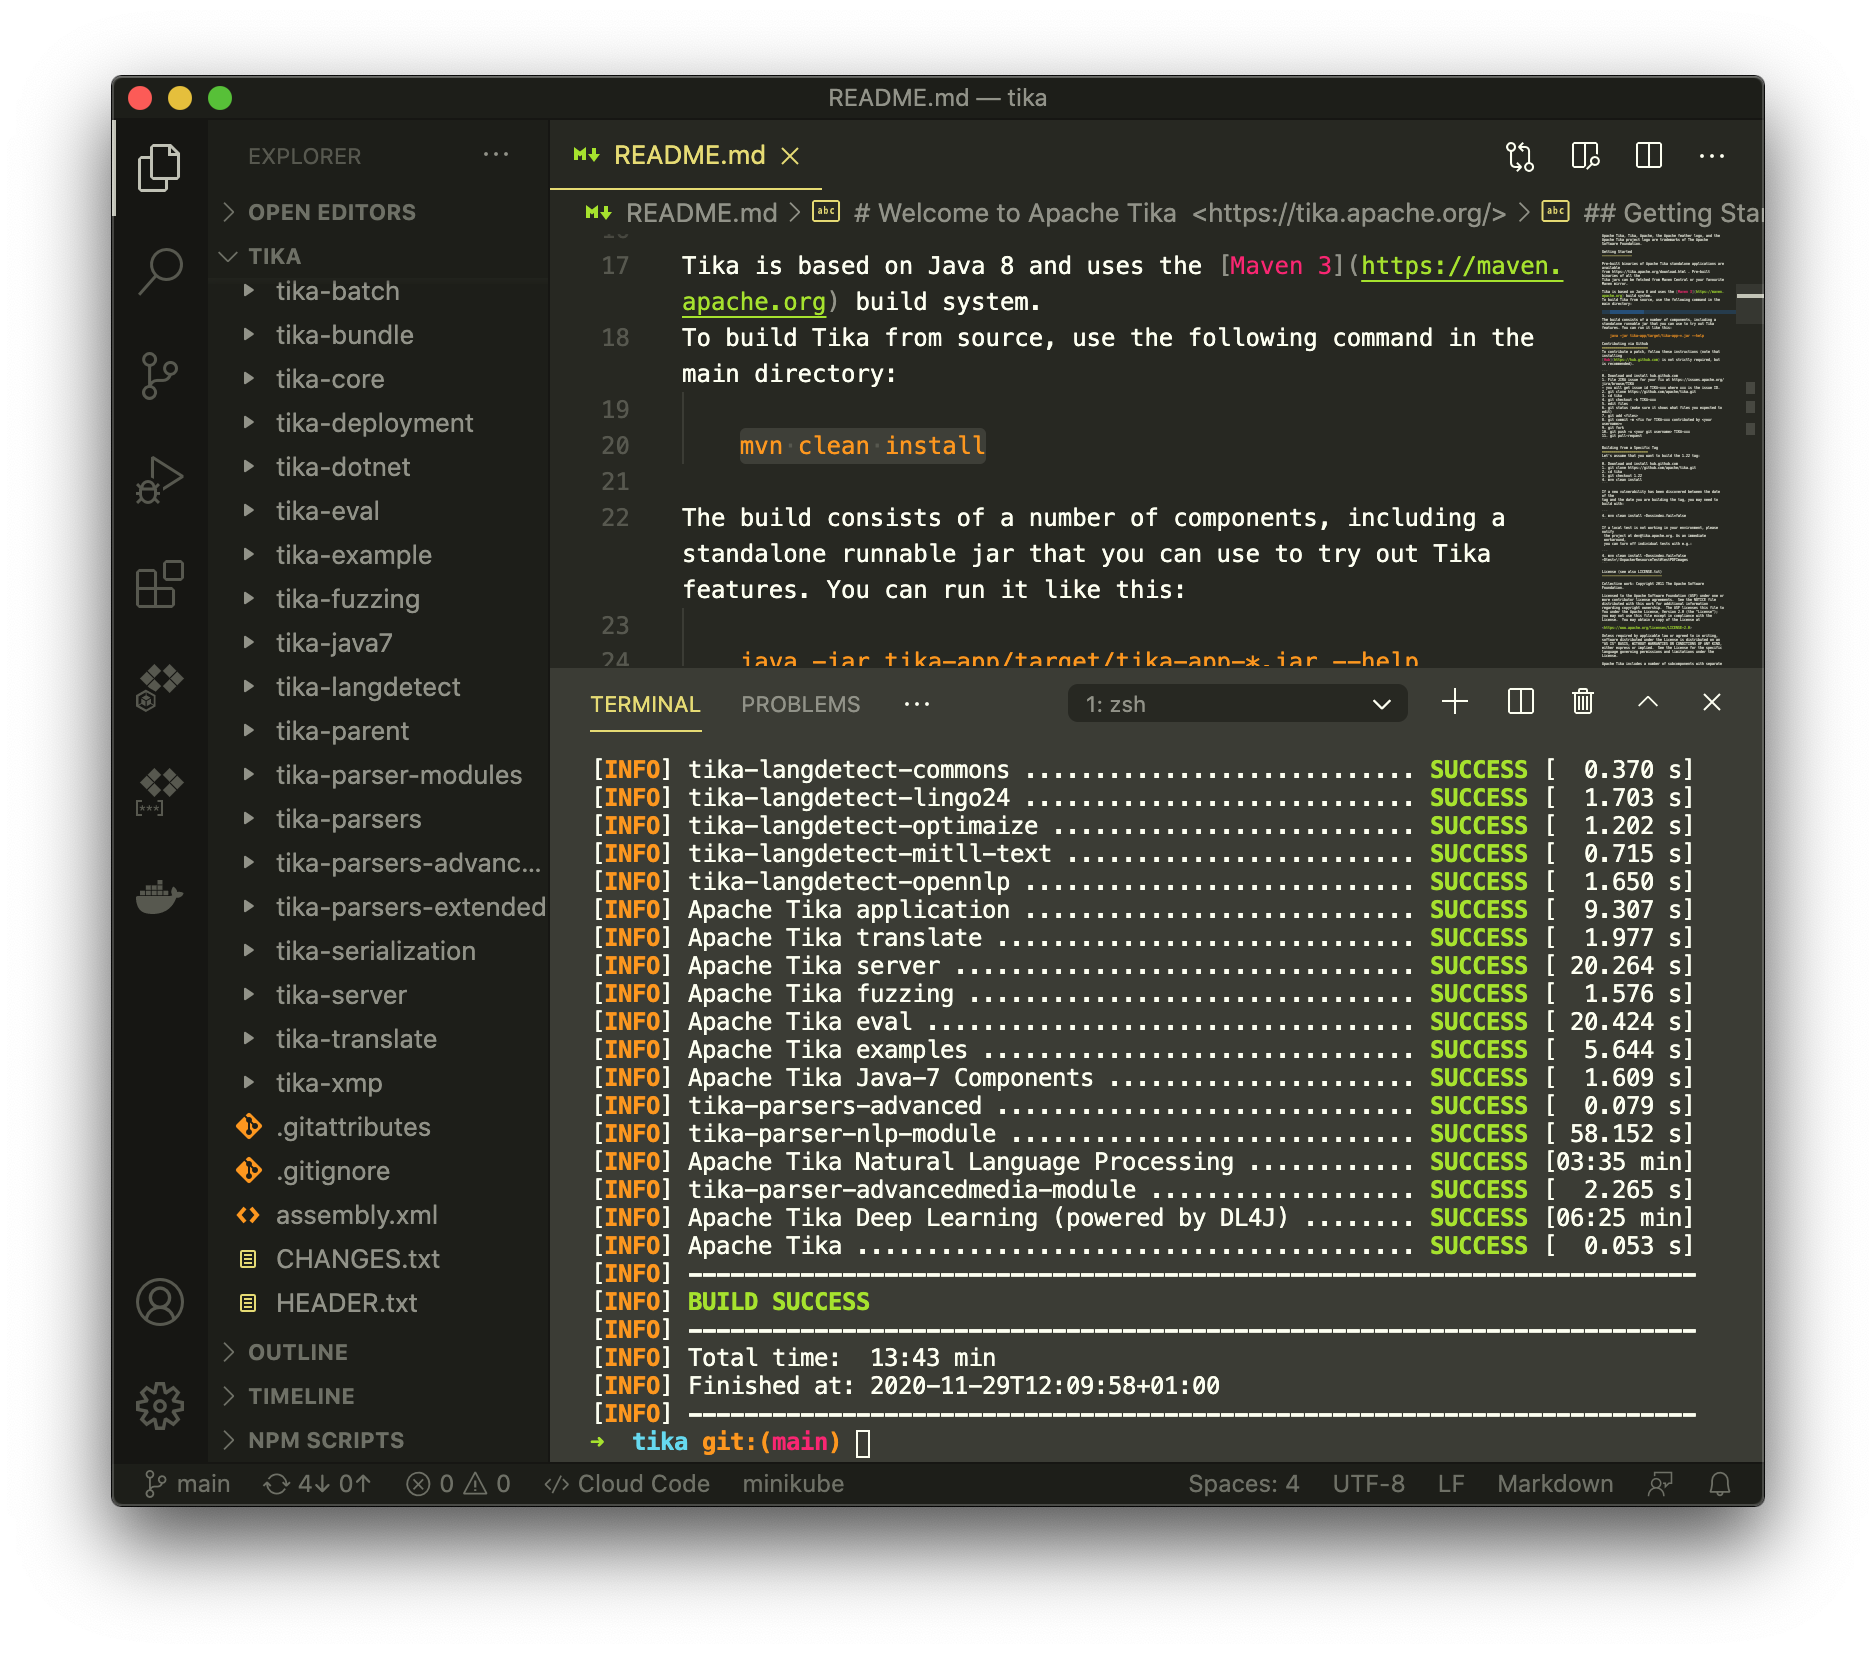
\includegraphics[width=0.85\textwidth]{report/images/compiling-tika.png}
    \caption{Apache Tika compilation.}
    \label{fig:compilation}
\end{figure}

\subsection{High-level overview}
We first ran the program byte-code through \textit{Structure101} \citep{chedgeystructure101}. See the composition graph, Figure~\ref{fig:composition}.

\newpage
\newgeometry{left=5mm, right=5mm}
\begin{figure}[ht]
    \centering
    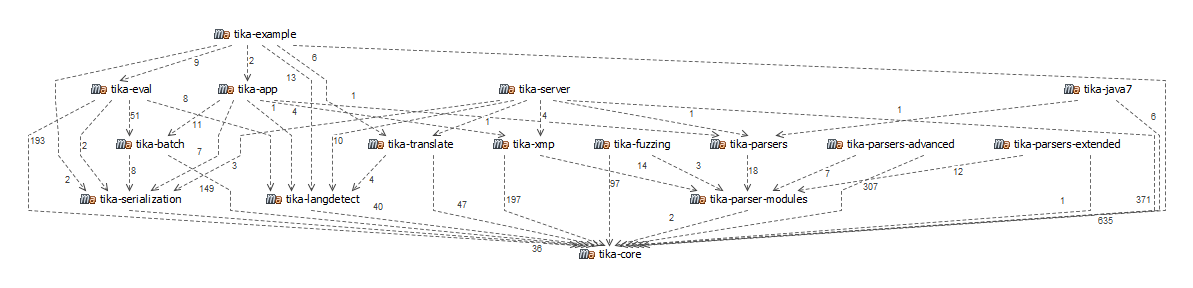
\includegraphics[width=1\textwidth]{report/images/tika.png}
    \caption{Composition Graph.}
    \label{fig:composition}
    
\end{figure}
\restoregeometry
\pagebreak

\subsection{Main components}
\subsubsection{tika-app}
The Tika interfaces: CLI and GUI. Allows users to interact with Tika in an interactive way. The GUI encapsulates the core and external parser libraries to build a single runnable jar file, which can be ran on multiple platforms as an user interface or via a command line interface. The program looks as can be seen in Figure~\ref{fig:tika_app/main}.

\begin{figure}[ht]
    \centering
    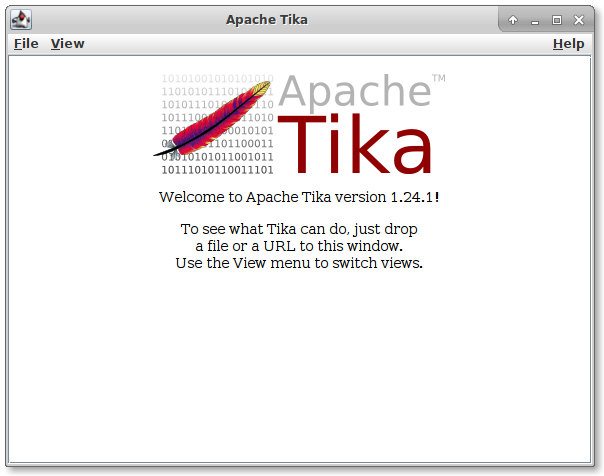
\includegraphics[width=0.85\textwidth]{report/images/tika_app/main.png}
    \caption{Apache Tika main GUI interface.}
    \label{fig:tika_app/main}
\end{figure}

To give an example of the tika-app layout and overall capabilities, we ran Tika on a web page of our choosing. The webpage we chose was the Course Information Nestor page for SME, for which Tika extracted meta-data but also tried to determine its main text content. See Figures~\ref{fig:tika_app/filechooser}-\ref{fig:tika_app/maincontent} to see the process visually. Tika managed to get a pretty good idea of the main page content, having extracted the text from the Nestor page correctly.

To get an idea of the dependency structure of \texttt{tika-app}, see Figure~\ref{fig:tika_app/s101-overview}. See below a description of the dependencies/dependents.
\begin{figure}[ht]
    \centering
    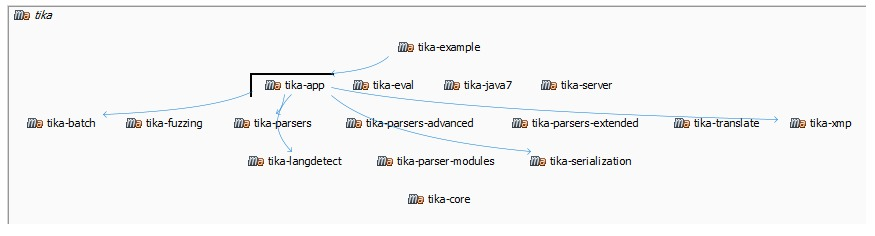
\includegraphics[width=0.85\textwidth]{report/images/tika_app/s101-overview.jpeg}
    \caption{Dependencies of \texttt{tika-app} in the overview of all Tika packages.}
    \label{fig:tika_app/s101-overview}
\end{figure}

\begin{itemize}
    \item \textbf{Dependencies}: \texttt{tika-parsers}, \texttt{tika-batch}, \texttt{tika-langdetect}, \texttt{tika-serialization}, \texttt{tika-xmp}.
    \item \textbf{Dependents}: \texttt{tika-example}
    \item \textbf{Internal structure}: See Figure~\ref{fig:tika_app/s101}. Three modules were tagged with a blue dot: \texttt{cli}, \texttt{gui} and \texttt{batch}. These are the main entry points to the module, and are all packed inside \texttt{tika-app.org.apache.tika}.
    \item\textbf{Purpose}: This component helps the users to interact with Tika and make use of its functionalities. It contains a simple and an easy to use interface which provides all Tika’s capabilities.
\item\textbf{Content}: Three modules were tagged with a blue dot: \texttt{cli}, \texttt{gui} and \texttt{batch}. These are the main entry points to the module, and are all packed inside \texttt{tika-app.org.apache.tika}. These external interfaces, like the CLI and GUI, allow the end-users to communicate and use Tika into their applications. 

\end{itemize}

\subsubsection{tika-core}
This module packs Tika's core functionality. It includes a module to detect file content types, a framework for parsing (text) content from a file and more, like language detection and so forth.

To get an idea of the dependency structure of \texttt{tika-core}, see Figure~\ref{fig:tika_core/s101-overview}. See below a description of the dependencies/dependents.


\begin{figure}[ht]
    \centering
    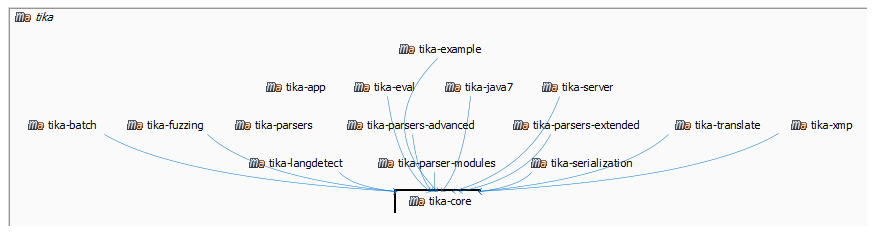
\includegraphics[width=0.85\textwidth]{report/images/tika_core/s101-overview.png}
    \caption{Dependencies of \texttt{tika-core} in the overview of all Tika packages.}
    \label{fig:tika_core/s101-overview}
\end{figure}

\begin{itemize}
    \item \textbf{Dependencies}: None
    \item \textbf{Dependents}: Every other package
    \textbf{directly} relies on \texttt{tika-core} except \texttt{tika-app} and \texttt{tika-parsers}. See Figure~\ref{fig:tika_core/s101-overview}.
   % \item \textbf{Internal structure}: See Figure~\ref{fig:tika_core/s101}. \texttt{tika-core} starts with the main \texttt{Tika} class, which requires a \texttt{Detector} and a \texttt{Parser} (and possibly a \texttt{Translator}) to build a \texttt{Tika} instance (also called \textit{Facade}) in the source code. This \texttt{Tika} class contains no main functionality itself, but rather calls on its dependencies (hence the word Facade).
    \item\textbf{Purpose}: This component represents the foundation on which other important components are constructed, like Tika app and Tika parsers. It consists of core interfaces and classes. 

\item\textbf{Content}: The core package consists of classes that build Tika facade, the mime package which is used for file format detection and the parser package used for parsing. All the other parser packages present in the overview in Structure 101 extend this package with extra capabilities. In addition, the language identifier mechanism, the metadata package and sax package are present in the core library and they are responsible for language analysis, metadata extraction and outputting structured text, respectively.

\end{itemize}

\subsubsection{tika-parsers}
\begin {itemize}
\item \textbf{Figure}: See Figure~\ref{fig:tika-parser}
\item \textbf{Dependencies}: \texttt{tika-parser modules}
\item \textbf{Dependents}: \texttt{tika-app, tika-java7, tika-server.}
\item \textbf{Purpose}: According to the documentation, Tika parsers are considered as key features that ensure the main functionalities of Tika. These parsers are responsible for parsing, understanding and processing all the existing file formats and their corresponding metadata models. Even though these tasks are intense and complicated, the parsers camouflage their complexity by providing a really simple tool to the users for extracting the needed text content.
\item \textbf{Contents}: This component consists of the tika parsers. Tika parsers are fundamental elements of Apache Tika. They contain a set of classes that construct the Tika Parser interface based on external parser libraries. 
\end{itemize}
\begin{figure}[ht]
    \centering
    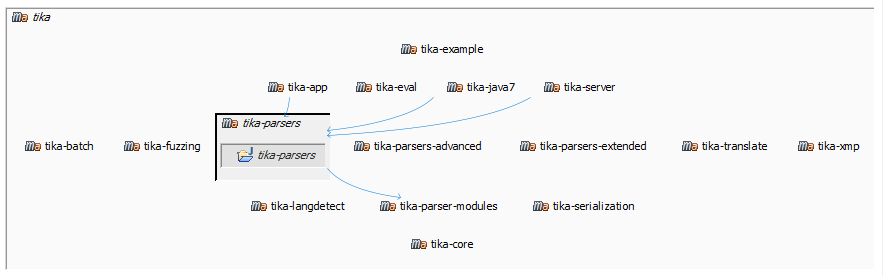
\includegraphics[width=1\textwidth]{report/images/tika-parser.PNG}
    \caption{tika-parser component}
    \label{fig:tika-parser}
\end{figure}
\subsubsection{tika-parsers-advanced}
\begin {itemize}
\item \textbf{Figure}: See Figure~\ref{fig:tika-parser-advanced}
\item \textbf{Dependencies}: \texttt{tika-core, tika-parser-modules.}
\item \textbf{Dependents}:  None
\item \textbf{Purpose}: Tika-parser-advanced is another crucial component that consists of several advanced parsers. These parsers provide more sophisticated functionalities and they are mainly focused on extracting more detailed information from complicated text documents like electronical clinical records, journals etc. 
\item \textbf{Contents}: This component offers extra parser functionalities and it consists of 4 modules. The first module is \texttt{tika-age-recognizer} and it is capable of detecting and extracting the ages of people in a given text. The second one is \texttt{tika-dl} and its main functionality is image recognition. \texttt{Tika-parser-advancedmedia-module} is another parser and it is responsible for captioning and recognizing objects present in images and graphics.  Finally, \texttt{tika-parser-nlp module} offers functionalities such as: parsing biomedical information, detecting locations in a given text and providing them geo tags based on latitude/longitude, extracting journal information etc.
\end{itemize}
\begin{figure}[ht]
    \centering
    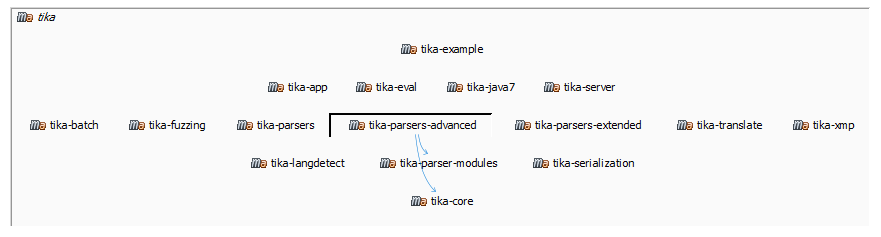
\includegraphics[width=1\textwidth]{report/images/tika-parser-advanced.PNG}
    \caption{tika-parser-advanced component}
    \label{fig:tika-parser-advanced}
\end{figure}
\subsubsection{tika-parsers-extended}
\begin {itemize}
\item \textbf{Figure}: See Figure~\ref{fig:tika-parser-extended}
\item \textbf{Dependencies}: \texttt{tika-parser-modules, tika-core}
\item \textbf{Dependents}: None
\item \textbf{Purpose}: This component is an extended version of the previously mentioned tika-parser components. It consists of additional parsers that are capable extra file formats.
\item \textbf{Contents}: This component consists of several parsers that provide additional capabilities. The first module is tika-parser-scientific-module and it parses extra file formats like NetCDF files, HDF files, geo file formats etc. The next module is tika-parser-sqlite3-module and it parses SQLite3 files. The last module is tika-parser-extended-integration-tests and it contains integration tests for Apache Tika.
\end{itemize}
\begin{figure}[ht]
    \centering
    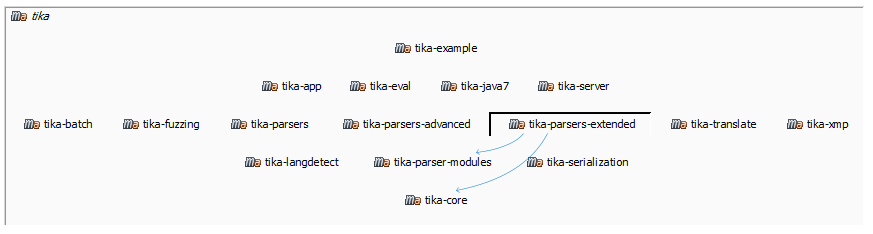
\includegraphics[width=1\textwidth]{report/images/tikaparserextended.PNG}
    \caption{tika-parser-extended component}
    \label{fig:tika-parser-extended}
\end{figure}
\subsubsection{tika-parsers-modules}
\begin {itemize}
\item \textbf{Figure}: See Figure~\ref{fig:tika-parser-modules}
\item \textbf{Dependencies}: \texttt{tika-core}
\item \textbf{Dependents}: \texttt{tika-fuzzing, tika-parsers, tika-parser-advanced, \\tika-parser-extended, tika-xmp}.
\item \textbf{Purpose}: This component provides the basic parsers that are mainly applied in common text file formats like Microsoft documents, PDF files etc. 
\item \textbf{Contents}: : This component contains multiple parser modules. One of these parser modules is \texttt{tika-parser-audiovideo-module} which parses audio and video metadata files. Another module is \texttt{tika-parser-cad-module} and it is responsible for searching for bits in the headers of the texts. In addition, \texttt{tika-parser-crypto-module} is another module that consists of parsers for PKCS7 data and for Time Stamped Data Envelope. There are also other parsers in this module that extract information from Microsoft documents, pdf files, mails, html pages, xml etc. 
\end{itemize}
\begin{figure}[ht]
    \centering
    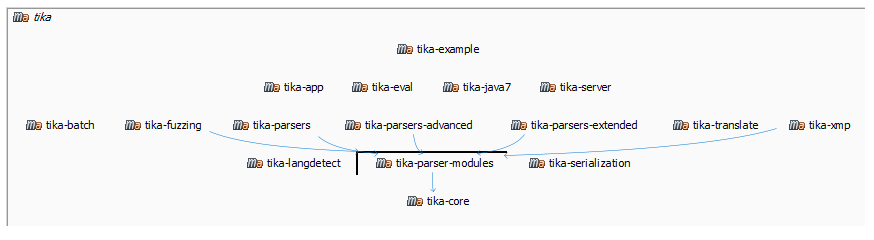
\includegraphics[width=1\textwidth]{report/images/tikamodules.PNG}
    \caption{tika-parser-modules component}
    \label{fig:tika-parser-modules}
\end{figure}
\subsubsection{tika-eval}
\begin {itemize}
\item \textbf{Figure}: See Figure~\ref{fig:tika-eval}
\item \textbf{Dependencies}:\texttt{ tika-batch, tika-langdetect, tika-core, tika-serialization.}
\item \textbf{Dependents}: \texttt{ tika-example.}
\item \textbf{Purpose}: The main purpose of this component is to provide insight based on the output of a given extraction tool or to perform comparisons between different tools. In addition, this component helps the developers to make comparisons of the output of two versions of the same tool or their execution while they run on different settings. 
\item \textbf{Contents}: Tika.eval consists of some elements. One of them is \texttt{eval.db} which stores the extracted content and the corresponding metadata. Another part in \texttt{tika.eval} is \texttt{tika.eval.textstats} and it contains interfaces that measure language probabilities and token stats.  In addition, \\\texttt{tika.eval.langid} contains the IDs of the languages. Tika.eval provides its own predefined list of reports where users can instantly report insights. 
\end{itemize}
\begin{figure}[ht]
    \centering
    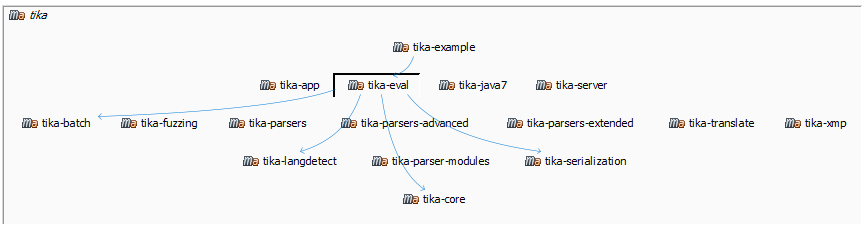
\includegraphics[width=1\textwidth]{report/images/tika-eval.PNG}
    \caption{tika-eval component}
    \label{fig:tika-eval}
\end{figure}
\subsubsection{tika-server}
\begin {itemize}
\item \textbf{Figure}: See Figure~\ref{fig:tika-server}
\item \textbf{Dependencies}: tika-parsers, tika-langdetect, tika-core, tika-serialization, tika-translate, tika-xmp.
\item \textbf{Dependents}: None
\item \textbf{Purpose}: Tika JAX-RS REST application. This is a Jetty web server running Tika REST services.
\item \textbf{Contents}: This component contains many classes that are responsible for maintaining and monitor the server of Tika. Some of these classes are: \texttt{serverstatus, servertimeout, taskstatus, tikaserverwatchdog} etc. All the classes of this component make sure that the server is running properly and executes its tasks correctly. In addition, they detect when something is wrong and notify the developers.
\end{itemize}
\begin{figure}[ht]
    \centering
    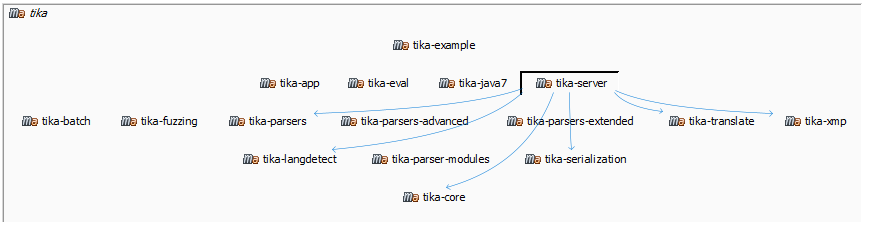
\includegraphics[width=1\textwidth]{report/images/tika-server.PNG}
    \caption{tika-server}
    \label{fig:tika-server}
\end{figure}
\subsection{Other components}
\begin{itemize}
    \item \texttt{tika-bundle} OSGi bundle that contains tika-core and tika-parsers as dependencies - but no code itself.
    \item \texttt{tika-example}. Contains some usage examples; including those shown on the \href{https://tika.apache.org/1.20/examples.html#Apache_Tika_API_Usage_Examples}{\underline{Usage Examples}} page. Is neither runnable nor meant to be directly used by another package. Because it contains examples resembling a diverse set of use cases, it is dependent on many other modules, i.e. \texttt{tika-app}, \texttt{tika-serialization}, \texttt{tika-translate},\\ \texttt{tika-langdetect-optimaize}, \texttt{tika-eval-core} and \texttt{tika-core}.
    \item \texttt{tika-fuzzing}. Contains very little documentation. Contains a \\ \texttt{AutoDetectTransformer} class that seems to take in an array of transformers and allows one to work with the entire vector of transformers at once.
    \item \texttt{tika-xmp}. Provides a "\textit{conversion of the Metadata map from Tika to the XMP data model}". XMP is a format for storing file metadata in a consistent way. The module contains a bunch of classes that facilitate XMP conversion from different formats, like OpenDocument, MSOffice and RTF. Is dependent on \texttt{tika-core} and some \texttt{tika-parser-} modules for processing Microsoft Office documents.
    \item \texttt{tika-serialization}. Contains some serializers and de-serializers for storing and retrieving metadata as JSON objects. Is dependent on \texttt{tika-core}, but really only uses interfaces from the package instead of actual functionality, namely \texttt{org.apache.tika.metadata.Metadata}; used working with Metadata objects in the module. 
    \item\texttt {tika-translate}: It represents an interface that provides translating services and it consists of multiple translators. One of these translators is MosesTranslator that uses Moses decoder for translations. Another translation service is CachedTranslator and it is responsible for saving a map of previous translations in order to not repeat translation requests. In addition, this component consists of YandexTranslator that provides a REST client implementation of Yandex Translate API. Among these translation services, this component also makes use of GoogleTranslator and MicrosoftTranslator.
    \item\texttt{tika-langdetect}: This component is capable of identifying the language of a given text. This type of information is quite helpful as a lot of metadata might not provide the language of the text formats. This component consists of a few language detectors like langdetect.lingo 24, langdetect.commons etc. 
    \item\texttt{tika-batch}: This module has the purpose of conventional processing and it has a producer/consumer design pattern. This module is still under development and the developers try to keep it as configurable as possible. It consists of a ResourceCrawler, which adds potential files for processing onto the queue. A ResourceConsumer is also present in the batch and it pulls a resource from the queue and consumes it. In addition, a StatusReporter often reports on how many files have been processed etc.
    \end{itemize}





\section{Identifying God Components}
To identify God Components, let us remind ourselves of the definition of a God Component. It is a software component whose Lines Of Code or number of classes got so extraneously large that the code got unmanageable. To find such components in our software, we need a tool to parse the entire code-base and infer the appropriate statistics from them. Probably, a tool written in Java would suit best, since it could use native methods to parse the code-base and thus reverse-engineer the software in an efficient way. A tool that is well suited for our purpose is \textit{Designite} \citep{sharma2016designite}. Designite is a quality assessment software tool that can be used to identify numerous technical debts in your software codebase. Among which, architectural smells and including God Components. Let us explain how we used this software to find God Components in Apache Tika.

\subsection{Designite}
Designite defines God Components in terms of lines of code and number of classes. The higher the amount of classes or lines of code, the more chance a component is considered as a God component. Designite classifies packages as a God Component if the package has more than 30 classes, or due to some other predefined condition which is less commonly encountered.

To test Designite functionality, we ran the tool on the latest version of the Tika git repository; at the time of writing \texttt{2.0.0-SNAPSHOT}. Having ran the Designite Enterprise edition, 15 God Components were identified (Figure~\ref{fig:designite-cli}).

\begin{figure}[ht]
    \centering
    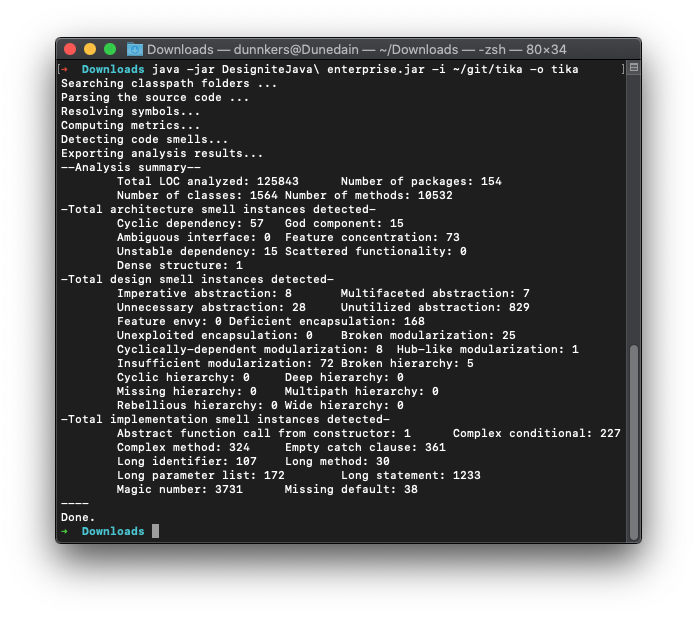
\includegraphics[width=0.8\textwidth]{report/images/designite/cli_analysis.png}
    \caption{Designite ran in a Terminal window. CLI shows a summary of the analysis. Extensive details of the analysis are stored in .txt files.}
    \label{fig:designite-cli}
\end{figure}

We can see that the codebase contains 125,843 Lines of Code (LOC) and has 10,532 methods spread over 1,564 classes packed up in 154 packages. This means the codebase is of reasonable size. Note these numbers apply only to the \texttt{2.0.0-SNAPSHOT} version of the code: the challenge now lies in running Designite for \textbf{all} versions of the code. More precisely said, the aim is to run Designite for every \textbf{commit} of the code: enabling us to analyze the evolution of God Components in the finest resolution possible. Let's build a script that runs Designite on every commit for us, automatically.

\subsection{Running Designite programmatically}
The relevant files for our Designite data-collection code are \texttt{find\_gcs.py} and a support file, \texttt{git\_utils.py}. Like their name imply, they are both Python scripts, where \texttt{find\_gcs.py} is dependent on the \texttt{git\_utils.py} module. Let us describe the step-by-step process of the entire operation.

\begin{enumerate}
    \item \textbf{Grabbing commits}. First, we need a list of commit ids (SHA-1 hashes) such that we can devise check out the specific version of the code one by one and run Designite on it. We do this, by running a \texttt{git log} command, with some \texttt{--pretty} modifiers to output the information in a desirable format. We then use the Python Pandas \citep{mckinney2011pandas} module to read in the information into a \textit{DataFrame}, a tabular datatype for storing large datasets. Columns that get stored include commit id, author name, commit date/time, commit message and the relevant Jira issue, if present in the commit message. The described functionality is described in the \textsc{get\_commits} function in \texttt{git\_utils.py}. Examples of some rows are as seen in Table~\ref{tab:commits-example}:
    
    \begin{table}[ht]
    \begin{tabular}{lllll}
    id                                       & author    & datetime                  & message                                       & jira      \\
    7f65d61 & THausherr & 2020-12-14 & TIKA-3248: revert accidental commit (2nd try) & TIKA-3248 \\
    326b7d7 & THausherr & 2020-12-14 & Revert "Merge origin/main into main"          & NaN       \\
    dd85c73 & THausherr & 2020-12-14 & Merge origin/main into main                   & NaN      
    \end{tabular}
    \caption{Commit data as mined by our application, stored in a Pandas Dataframe. Commit \textbf{time} was omitted from the 'datetime' column for brevity.}
    \label{tab:commits-example}
    \end{table}
    
    Note there also is an example of the resulting DataFrame in the \texttt{statistics.ipynb} Notebook in the root folder of our repo.
    
    \item \textbf{Running Designite}. Next, we loop each commit and run Designite from the Python script using \texttt{os.system} - a function used to execute terminal commands. Once Designite finished running, it outputs \texttt{.csv} files to some chosen directory. We take the relevant file (\texttt{ArchitectureSmells.csv}), extract the God Components, and again output that information to a .csv file of our own. The data also has its columns renamed and some transformed for easier data processing down the line: the reason why Designite classified the component as a GC is extracted, for example, along with the relevant metric, like \# classes. See Table~\ref{tab:designite-output}:
    
    \begin{table}[ht]
    \begin{tabular}{llllll}
    commit                                   & repo         & package                 & smell         & cause         & metric \\
    49bb469 & tika-cpu\_21 & org.apache.tika.example & God Component & MANY\_CLASSES & 49     \\
    49bb469 & tika-cpu\_21 & org.apache.tika.batch   & God Component & MANY\_CLASSES & 31     \\
    49bb469 & tika-cpu\_21 & org.apache.tika.detect  & God Component & MANY\_CLASSES & 31    
    \end{tabular}
    \caption{Designite output data, captured per-commit and with the '\# classes' metric processed into a separate column.}
    \label{tab:designite-output}
    \end{table}
    
    For memory purposes, we remove the other, irrelevant Designite reports. The relevant code for this step is found in \texttt{find\_gcs.py}.
\end{enumerate}

We are now able to run Designite for all commits in the Tika project! That's great. But, because the Tika repository has nearly 5,000 commits, we would have to run Designite around 5,000 times. With an average runtime of about 40 seconds, it is easy to see that the computational complexity got quite large and the problem would take quite a while to run on one CPU, around 55 hours of running Designite non-stop. This might be a bit infeasible to do on just simple Laptops. Therefore, we utilized the University's High-Performance Computing cluster \textit{Peregrine} to solve the problem.

\subsection{Running Designite on Peregrine}
\textbf{Peregrine} is a HPC cluster containing computational nodes for several purposes. Our goal is to speed up the Designite running process, which requires a working copy of the Tika repository to check out a certain version (commit) of the code. On Peregrine, we have access to at least 24 CPU's in a single node. The idea we implemented was to run Designite simultaneously on each of the 24 CPU's available to us in the HPC environment. This also means, however, that we also need 24 working copies of the Tika repository. Dependent on the exact Tika version checked out, the repository comes in at around 2 GB. During the process of running Designite, the entire code-base will be loaded up into memory. So, theoretically this would add up to around 48 GB. In practice, however, much more memory is needed to load up 24 copies of Tika in Designite at the same time: there's probably some memory overhead in storing certain Data types and making the necessary computations and inferences. We therefore fall short on memory when utilising a 'regular' Peregrine node, which has 128 GB memory available. Luckily, however, Peregrine has '\textbf{high memory}' nodes available to us.

The high memory nodes allow us to set up to 1,024 GB (1 TB) of working memory, available to all our cores. Using this gigantic amount of memory, we were able to run Designite on 24 versions of the code simultaneously. Even though the queue time for this node is quite long, we only have to go through this process once, if we do it well. So let's see how we architected the parallel structure in the code.

On every run, the commits that had no Designite run yet, are mapped over the available CPU's. Then, the \textsc{clone\_tika} function in \texttt{git\_utils} makes sure that every CPU has its own clone of the Tika repository. To make sure each run of Designite is ran on a clean version of the repo, \texttt{git clean} is used, among others. Having ran the entire operation on Peregrine, we receive a log output file that has the summary as seen in Listing~\ref{code:peregrine-output}.

\begin{lstlisting}[caption={Peregrine job output.}, label={code:peregrine-output}]
Peregrine Cluster
Job 16174792 for user 's2995697'
Finished at: Wed Dec 16 02:40:31 CET 2020

Job details:
============

Job ID              : 16174792
Name                : sme_god-components
User                : s2995697
Partition           : himem
Nodes               : pg-memory05
Number of Nodes     : 1
Cores               : 24
State               : COMPLETED
Submit              : 2020-12-15T10:17:59
Start               : 2020-12-15T21:08:07
End                 : 2020-12-16T02:40:29
Reserved walltime   : 2-22:00:00
Used walltime       :   05:32:22
Used CPU time       : 5-10:36:50 (efficiency: 98.25%)
% User (Computation): 91.59%
% System (I/O)      :  8.41%
Mem reserved        : 1000G/node
Max Mem used        : 124.29G (pg-memory05)
Max Disk Write      : 153.60K (pg-memory05)
Max Disk Read       : 7.65M (pg-memory05)
\end{lstlisting}

It can be observed that our job ran with high efficiency (98.25\%), indicating we put all nodes at work nicely. The maximally used amount of memory comes in at 124 GB, indicating we only barely topped out the 128 GB memory available to us on regular Peregrine nodes. Apparently, no memory can be allocated already before the job report says to have used 128 GB memory. In all, it took the job more than 5 hours to complete, giving us a nice speedup on the sequential operation. That said, once this massive operation is complete, we simply take all the separate .csv files and concatenate them into one huge result file. This file is stored in \texttt{output/all\_reports.csv}.

\subsection{Data analysis}
Now that we have a huge data file, we need to analyze it. This is done in the Jupyter Notebook \texttt{statistics.ipynb}. We are able to iterate every commit and decide figure out what God Components exist in that version of the code. It is important, we do not make assumptions about the starting- and ending dates of the God Components; a component might become a GC and stop being one multiple times. Having aggregated all this data into a suitable data frame, we obtain the Figure~\ref{fig:gc_lineplot}.

\begin{figure}[ht]
    \centering
    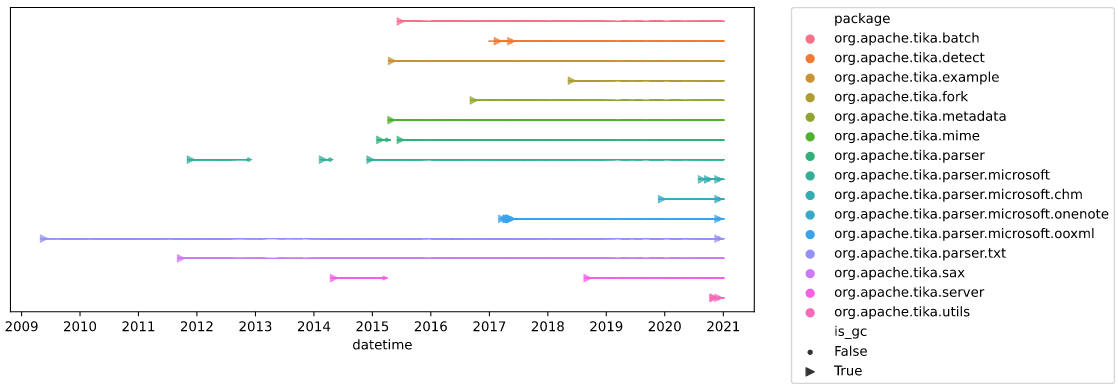
\includegraphics[width=\textwidth]{report/images/gc_lineplot.png}
    \label{fig:gc_lineplot}
    \caption{All God Components shown such that all their GC 'starting'- and 'ending' dates are visible; when they became a GC and when they stopped being one.}
\end{figure}

Interesting insight. It can be seen that there were in total 15 God Components detected throughout the existence of the Tika codebase. Some of which have stopped being a GC in between, having a break of sometimes up to a couple years before becoming a GC again (tika.server). However, we should note that some GC's have shorter breaks, sometimes so short that the line in the plot is still continuous - the re-emergence of the GC in that case can be seen by the caret indicator ($\blacktriangleright$).

What would also be interesting, however, is to discover what commits added/removed code to some God Component. For this, we have our final part of the code: the \textsc{compute\_locs} function in \texttt{git\_utils.py}. \textsc{compute\_locs} uses \texttt{git diff} to discover what files changed for some certain commit. The output is then formatted and loaded up into a Pandas data frame for further analysis. For every file changed in some commit, we found out whether it affected some God Component; we do this by checking whether the package name exists in the path. An example match would be \texttt{tika/tika-core/src/main/java/org/apache/tika} $\Leftrightarrow$ \texttt{org.apache.tika}. More specifically, packages that have higher levels of nesting are tested on a match first, i.e. \texttt{org.apache.tika.parser} will be tested before \texttt{org.apache.tika} because its nesting level is higher. Only the first match is taken into consideration - preventing multiple packages matching just one file. For an example of how this processed data looks like, see Table~\ref{tab:locs}:

\begin{table}[ht]
\begin{tabular}{llllllll}
additions & deletions & godcomp                          & id                                       & author    & ...\\
1         & 3         & org.apache.tika.batch            & 7f65d61 & THausherr & ... \\
8         & 14        & org.apache.tika.parser           & 7f65d61 & THausherr & ... \\
2         & 3         & org.apache.tika.parser.microsoft & 7f65d61 & THausherr & ... \\
\end{tabular}
\caption{Lines Of Code added/removed information captured per-commit, for each God Component that was found to have its files modified by the commit. Note some commit information was omitted for brevity sake.}
\label{tab:locs}
\end{table}

With all per-commit info from git diff mapped to a God Components, we can map the total Lines Of Code (LOC) that each commit builds up to each God Component. This mapping operation of computing the cumulative LOC's over time space is done in the \texttt{statistics.ipynb} file. See Figure~\ref{fig:loc_growth} for the result.

\begin{figure}[ht]
    \centering
    \includesvg[width=\textwidth]{report/images/god_components/gcs-package-loc-growth.svg}
    \label{fig:loc_growth}
    \caption{God components growth in Apache Tika. X-axis represents the time and Y-axis represents the lines of code, in \textbf{logarithmic scale}.}
\end{figure}

Note that the y-axis is in logarithmic scale: the differences in LOC buildup between the various GC's was too large to make a nice chart otherwise. It is important to take this fact into account when interpreting the chart - in terms of Lines Of Code, by far the biggest component is \texttt{org.apache.tika.parser}. When carefully inspecting the chart, it can be seen that that component is really an order of magnitude larger than the other ones, i.e. others compare at around 10,000 LOC at the time of writing, compared to the parser's around 100,000 lines. That's a big difference. Let us now explore some specific God Components in more depth.

\section{God Component Analysis}
This section focuses on performing an analysis towards the identified God components. The analysis is built based on answering the following questions: \textit{What types of issues contributed to the creation of God components? How many developers contribute to God components? What types of issues contributed to the re-factoring of God components? How long do God components stay inside a system?} All these questions provide us with insight regarding the evolution of God Components in Tika.

As mentioned in the previous section, Designite was used as a tool for identifying the God components within Tika. This tool is capable of recognizing the God components based on lines of code and number of classes. If a package has more than 30 classes, then it is classified as a God component.\\
After analyzing the code, Designite identified 15 God components through all the versions of Tika. These God components are listed below and visualized in the plots which demonstrate the growth of these components in terms of number of classes and lines of code. See Table~\ref{tab:gc-summary} for a summary of all found GC's and some general statistics about them.

\begin{table}[ht]
\begin{tabular}{lllll}
package                                  & Became GC at & \# commits & \# days & \# authors \\
org.apache.tika.batch                    & 2015-06-28   & 2352          & 1996       & 114        \\
org.apache.tika.detect                   & 2017-01-19   & 1579          & 1424       & 82         \\
org.apache.tika.example                  & 2015-05-04   & 2433          & 2050       & 115        \\
org.apache.tika.fork                     & 2018-05-31   & 738           & 927        & 52         \\
org.apache.tika.metadata                 & 2016-09-26   & 1743          & 1539       & 88         \\
org.apache.tika.mime                     & 2015-05-02   & 2443          & 2053       & 115        \\
org.apache.tika.parser                   & 2015-02-21   & 2429          & 2123       & 116        \\
org.apache.tika.parser.microsoft         & 2011-11-25   & 3052          & 3306       & 121        \\
org.apache.tika.parser.microsoft.chm     & 2020-08-21   & 155           & 114        & 14         \\
org.apache.tika.parser.microsoft.onenote & 2019-12-16   & 305           & 363        & 26         \\
org.apache.tika.parser.microsoft.ooxml   & 2017-03-23   & 1454          & 1361       & 80         \\
org.apache.tika.parser.txt               & 2009-05-22   & 4539          & 4223       & 123        \\
org.apache.tika.sax                      & 2011-09-25   & 3691          & 3367       & 121        \\
org.apache.tika.server                   & 2014-05-07   & 1078          & 2412       & 47         \\
org.apache.tika.utils                    & 2020-10-31   & 86            & 44         & 8         
\end{tabular}
\caption{Summary information of all found God Components in the Apache Tika codebase, across all different commits on the \textit{main} branch. All God Components are still a God Component to this day. The column '\# commits' denotes the amount of commits made to that God Component in its entire lifetime, i.e. even before being a God Component. '\# days' denotes the amount of days that component has been a God Component for, in total (i.e. the component may have stopped being a GC and then again continued to be a GC over its lifetime). Data applies to commits up till 14th of December 2020.}
\label{tab:gc-summary}
\end{table}


\begin{figure}[ht]
    \centering
    \includesvg[width=\textwidth]{report/images/god_components/gcs-package-classes-growth.svg}
    \label{fig:class_growth}
    \caption{God components growth in Apache Tika. X-axis represents the time and Y-axis represents the number of classes.}
\end{figure}

Next, we will discuss some individual God Components to do a more in-depth analysis. \texttt{org.apache.tika.parser}, \texttt{org.apache.tika.server} and \texttt{org.apache.tika.parser.txt} are chosen for this purpose.

\subsection{org.apache.tika.parser}
\begin{itemize}
    \item What types of issues contributed to the creation of God components? \\
    According to the Jira issue tracker, the developers of Tika contributed towards the system mainly in 4 aspects: improving the package, adding new features and functionalities, fixing existing bugs or issues and completing multiple tasks. More precisely, there are approximately 1200 commits regarding bug fixes, nearly 600 commits related to improving the package, almost 150 commits for adding features and 170 commits for task completion. The rest of commits have been created for testing, wish list purposes or sub-task completion. It is quite clear that the highest proportion of these commits are associated to bug fixes. These bug fixes have made the developers to create more code, to produce more lines of code and more packages as a result. This has lead to the creation of parser as a God component. 
    \item How many developers contribute to God components?\\ In total, there are 2429 commits regarding the parser God component and there is a total amount of 116 developers that contributed towards its evolution. Though out the commits, the developers improved different parts of the God component, added new features, fixed multiple bugs and worked on tasks and sub tasks.  
     \item What types of issues contributed to the re-factoring of God components?\\
    \item How long does this God component stay inside a system?\\ This package became a God component in 2015 and it still continues to be one. This implies that this package has been a God component for approximately 6 years. The parsers are key functionalities in the system of Tika, as they are responsible for extracting the content of the files and their corresponding metadata. It makes sense why this package is a God component and why it keeps evolving.

\end{itemize}

\subsection{org.apache.tika.server}
\begin{itemize}
    \item What types of issues contributed to the creation of the God components\\
    There are three main issues that had a significant influence on the evolution of tika.server. Two of these issues transformed this package into a God component, while one issue removed the tika.server from the list of the God components. The first issue (under Tika-2725) was mainly concerned with making the server robust against ooms(out of memory), infinite loops and memory leaks. This issue was defined as a task with a major priority and it made the tika.server as a God component. The second issue (under TIKA-1564) was mainly concerned with organizing the structure of tika.server package. It was defined as an improvement with minor priority. However, it had a huge impact on the package, as the package stopped being a God component. The last issue (under TIKA-1270) was mainly concerned with providing endpoints to JAX-RS server in form of "--list-$<>$" similar to the CLI. This issue was considered as an improvement with major significance, but did cause tika.server to become a God component again.\\
    Even though these issues helped in recognizing tika.server as a God component and determining when it was not, there are other issues that contributed in the creation or the removal of this God Component. Before the TIKA-2725 issue, there were a lot of major priority bugs that needed to be fixed like setting classpath for tika-server and opennlp processor models (TIKA-2713) or the server not being able to recognize http 3xx error codes when passing fileUrl (TIKA-2724) etc. Apart from issue TIKA-1654, there were other issues that contributed into the removal of the package from the God components. Based on Jira, there were a lot of changes and improvements happening in the server package like the server started functioning on Docker (TIKA-1518), there was a new tika-server front-end (TIKA-1545) and more cleanup of the code(TIKA-1556).
    \item How many developers contribute to the God component?
    In total, there are 2412 commits regarding the tika.server God component and there is a total amount of 47 developers that contributed towards its evolution. The issue that initially made the package a God component in 2014 was created by Nick Burch. %Other developers that contributed towards the creation of this God component are: Sergey Beryozkin, Chris A. Mattmann, Ali Mosavian. 
    In 2015, the package was not a God component any more. The issue that removed this package from the God components was created by Tyler Palsulich. Another developer that contributed to its removal is Tim Allison. In 2018, the package became a God component again. The issue that remade the package a God component was created by Tim Allison. %Other developers that contributed towards its creation are: Badger, Daniel La, NW Brad, Nick Burch.


    \item What types of issues contributed to the re-factoring of the God components?\\
    Most of the issues mentioned in the first question had a re-factoring effect in the tika.server package. One important issue that had a big influence in the package was TIKA-1564. The issue was mainly concerned with organizing and re-structuring the entire package.
    \item  How long does this God component stay inside the system?\\
    According to the graph, tika.server is one of the components that has had an interesting evolution. Initially, this package became a God component in May of 2014 and it continued being one till March of 2015. The package was removed from the God components until August of 2018. That is when tika.server started again being a God component and it continues to be one up to now. This package has been a God component within the system for approximately 3.5 years.
\end{itemize}


\subsection{org.apache.tika.parser.txt}

\begin{itemize}
    \item	What types of issues contributed to the creation of the God component?\\
    
    Similarly to the previously discussed package, there are 2 identified issues that caused significant changes to the parser.txt component. The first issue (under TIKA-233) was mainly concerned with using a smaller component of ICU4J library. It was considered as an improvement type of issue with a minor priority and it transformed this package into a God component. According to Jira, this occurred as a result of a large number of copies of relevant classes from ICU4J library. The second issue is quite unique, because it initially managed to remove this package from the God components, but within the timespan of a few hours it managed to remake the package a God component. The issue is defined as a task of major importance and it is mainly focused on clarifying the structure of parser module. The issue is still unsolved.\\
    Even though these issues had a quite significant impact on the evolution of this God component, there have been other issues that contributed in the creation or the removal of this God Component. Before the TIKA-233 issue, most of these issues were related to bug fixes and adding new features into the parsers. Some of them were mainly concerned with adding parser readers (TIKA-143), adding parsers for zip files (TIKA-149), adding parsers for XHTML content or fixing bugs like Missing body in HtmlParser. All these examples of issues show that this was the stage where all the parsers started being implemented in order to provide extra functionalities to Apache Tika. In addition, there are some other issues timely close to TIKA-3241 that contributed to removing and re-adding this package as a God component. Some of these issues were mostly bug of major importance like checking causes of tika exceptions when using  Tika library AutoDetectParser (TIKA-3243, RTFParser fails to generate full content of an RTF file (TIKA-3238), ForkParser displays incorrect message when parse timeout is reached (TIKA-3220). All these bugs still remain unresolved.
    \item How many developers contribute to the God component?\\
    In total, there are 4539 commits regarding the parser.txt God component and there is a total amount of 123 developers that contributed towards its evolution. The issue that initially made the package a God component in 2009 was created by Jukka Zitting, while the issue that removed the package from the God components and instantly remade it a God component was created by Tim Allison. \\
    \item	What types of issues contributed to the re-factoring of God components?\\
    The re-factoring issues that mainly influenced the God component were  the issues that were mainly concerned with improving the quality of the code of the component (improvements). One issue like this was TIKA-3179, which was of critical importance. The issue was mainly concerned with cleaning the parser’s hierarchy and restructuring the entire component. According to Jira comments, a lot of parsers were moved to new packages and the parser.extended package was also created for this issue.\\
    \item How long do God components stay inside a system?\\
    According to the graph, parser.txt is another component that has had an interesting evolution. It started being a God component in May of 2009 and it continued being one till December of 2020. However, the package had a strong comeback and it was reconsidered as a God component only a few hours after it was removed from the God components. In total, the God component has been present in the system for approximately 11 years.
    
\end{itemize}

\section{Commits and issues analysis}
This section focuses on analysing and describing some chosen issues in more details. Initially, a set of issues that contributed in the creation of the God components is chosen. After that, we analyze these issues in order to determine the possible rationale of the developers when it comes to adding or removing these God components. The analysis is performed based on the following questions:
\begin{enumerate}
\item Do developers discuss God components within issues? If yes, what do they discuss?
\item How do developers re-factor God components?
\end{enumerate}
\subsection{Issues}
For analyzing purposes, we have chosen different issues that are related to all the packages and classes that are defined as God components. \\
\textbf{TIKA-1663}
\begin{itemize}
    \item Do developers discuss God components within issues? If yes, what do they discuss?\\
    This is an improvement type of issue with a minor priority. It is mainly concerned with adding a DigestingParser to add MD5/SHA-X hashes as fields in Metadata. In the comment section, there is no specific mention neither of the god component itself nor the fact that the tika.batch package has a growing number of classes and LOC. The developers are mainly discussing about options on which Digest algorithms to use and how to implement them.  In addition, they discuss about adding parser decorators.
    \item How do developers re-factor God components?\\
    They re-factor this god component based on what was decided in the comment section. The developers agreed to enhance tika configuration framework and the parsers to accept runtime arguments. In this way, the developers could just declare the digest algorithm in the configuration file and the digestparser could easily use it without modifying any code of the applications. In addition, they implement more decorators by adding extra classes.
\end{itemize}

\textbf{TIKA-2273}
\begin{itemize}
    \item Do developers discuss God components within issues? If yes, what do they discuss?\\
    This is an improvement type of issue and it has a minor priority. It concerns tika.detect and it focuses on finding an easier configuration for encoding detectors through tika.config file. While they were trying to resolve the issue, one of the developers broke two tests in tika.bundle package and the other were trying to fix those. So, they only discuss about the broken tests. The developers are not discussing the God component.
    \item{itemize}	How do developers re-factor God components?\\
    The developers are not providing any information about re-factoring the component, as they mainly focused on fixing the broken test issues.
\end{itemize}

\textbf{TIKA-1562}
\begin{itemize}
    \item Do developers discuss God components within issues? If yes, what do they discuss?\\
    This is a bug issue and it is considered as of major importance. The issue concerns the tika.example package and it focuses on adding examples from the software into the “Tika in Action” book. The developers in the comment section are mainly discussing on what to include in the book. Specifically, they agree on adding a case studies section, where they explain when to use tika. This issue is concerned with editing the book. There is no specific mention of the god component. 
    \item How do developers re-factor God components?\\
    The developers are only discussing about “Tika in Action” book and what to add into the book, like examples for Tika use. There is no refactoring regarding the god component.
\end{itemize}

\textbf{TIKA-2653}
\begin{itemize}
    \item Do developers discuss God components within issues? If yes, what do they discuss?\\
    This issue is considered as a new feature, which is of major importance. It mainly concerns the fork parser and it focuses on letting the user to define a jar directory for class loading in the fork parser. Specifically, the developer attempts to make the process of using the fork parser easier for the users by making them depend only on tika.core. In addition, the developer aims to remove all the dependencies into a separate directory.  Even though this issue does not have any direct mention of the God component, the developers are trying to restructure the parser and many dependencies.
    \item{itemize}	How do developers re-factor God components?\\
    The developers are re-factoring the god component by restructuring the component, its hierarchy and possibly eliminating some of the dependencies.  
\end{itemize}

\textbf{TIKA-2057}
\begin{itemize}
    \item Do developers discuss God components within issues? If yes, what do they discuss?\\
    This is an improvement type of issue and it has a minor priority. It concerns the metadata and it focuses on extracting PDF DocInfo fields into separate metadata fields. The developers explain that when a PDF file is transformed into HTML, the metadata does not have any access to the title of the PDF file. There is no mention of the God component. The developers are only discussing on fixing this issue. 
    \item How do developers re-factor God components?\\
    The developers refactor only the metadata by  adding other DublinCore keys into it in order to get the DocInfo information.
\end{itemize}

\textbf{TIKA-1571}
\begin{itemize}
    \item Do developers discuss God components within issues? If yes, what do they discuss?\\
    This is an improvement type of issue of major importance. It concerns the parser package specifically the mime functionality. The issue is about upgrading the UCAR dependencies to java library version 4.5.5. The new version of the library provided some good bug fixes and improvements and the developers were agreeing on using them on their code. The developers do not mention anything about the growing amount of LOC.
    \item How do developers re-factor God components?\\
    The developers implemented a patch about an API deprecation and they tested it. There is no re-factoring of the component.
\end{itemize}

\subsection{Rationale}
Based on the analysed issues, it has been noticed that the developers mainly focus on solving the existing issues as efficient as possible. The developers are indeed concerned about the growing packages and components and there are some improvement type of issues that fix the structure and the hierarchies of the God components, after being resolved. However, it seems that the developers are mainly paying their attention to fixing the present issues, regardless of the fact that their solutions add up more lines of code. 
\bibliographystyle{plain} % We choose the "plain" reference style
\bibliography{report/bibliography}

\appendix
\section{Appendix: Analysis}
\subsection{Component overview}
\subsubsection{tika-app}
\begin{figure}[ht]
    \centering
    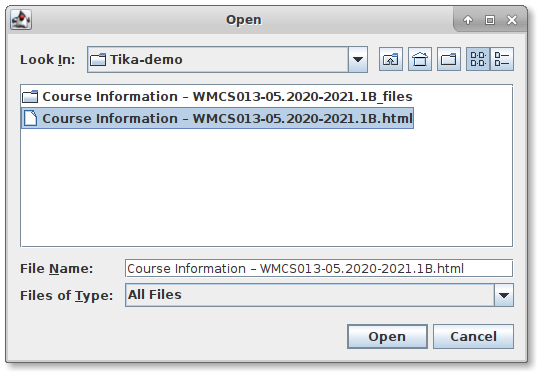
\includegraphics[width=0.85\textwidth]{report/images/tika_app/filechooser.png}
    \caption{Apache Tika app file choosing.}
    \label{fig:tika_app/filechooser}
\end{figure}
\begin{figure}[ht]
    \centering
    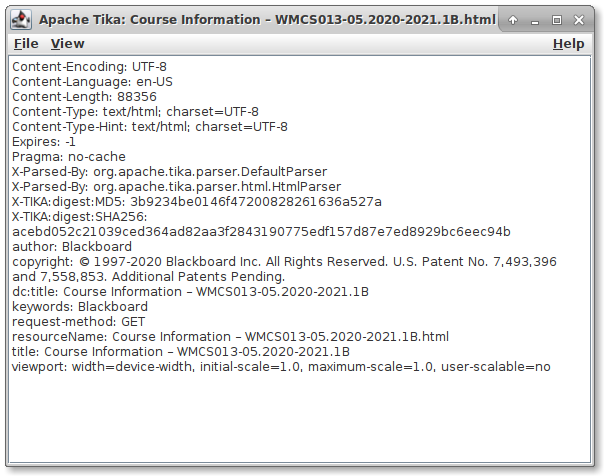
\includegraphics[width=0.85\textwidth]{report/images/tika_app/metadata.png}
    \caption{Extracted metadata from a HTML file. We chose the Course Information Nestor page.}
    \label{fig:tika_app/metadata}
\end{figure}
\begin{figure}[ht]
    \centering
    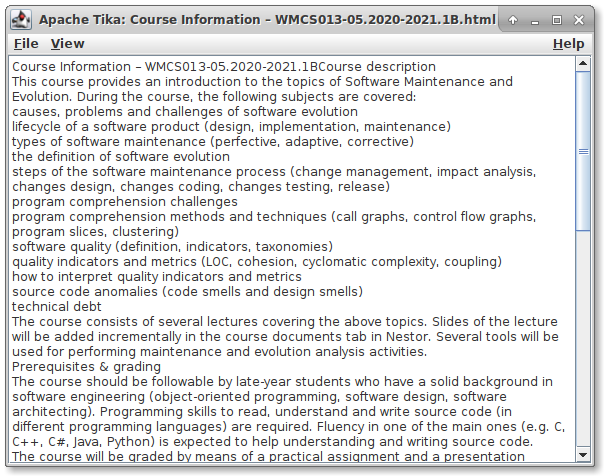
\includegraphics[width=0.85\textwidth]{report/images/tika_app/maincontent.png}
    \caption{Rendered main content from Tika's analysis using the app.}
    \label{fig:tika_app/maincontent}
\end{figure}
\begin{figure}[ht]
    \centering
    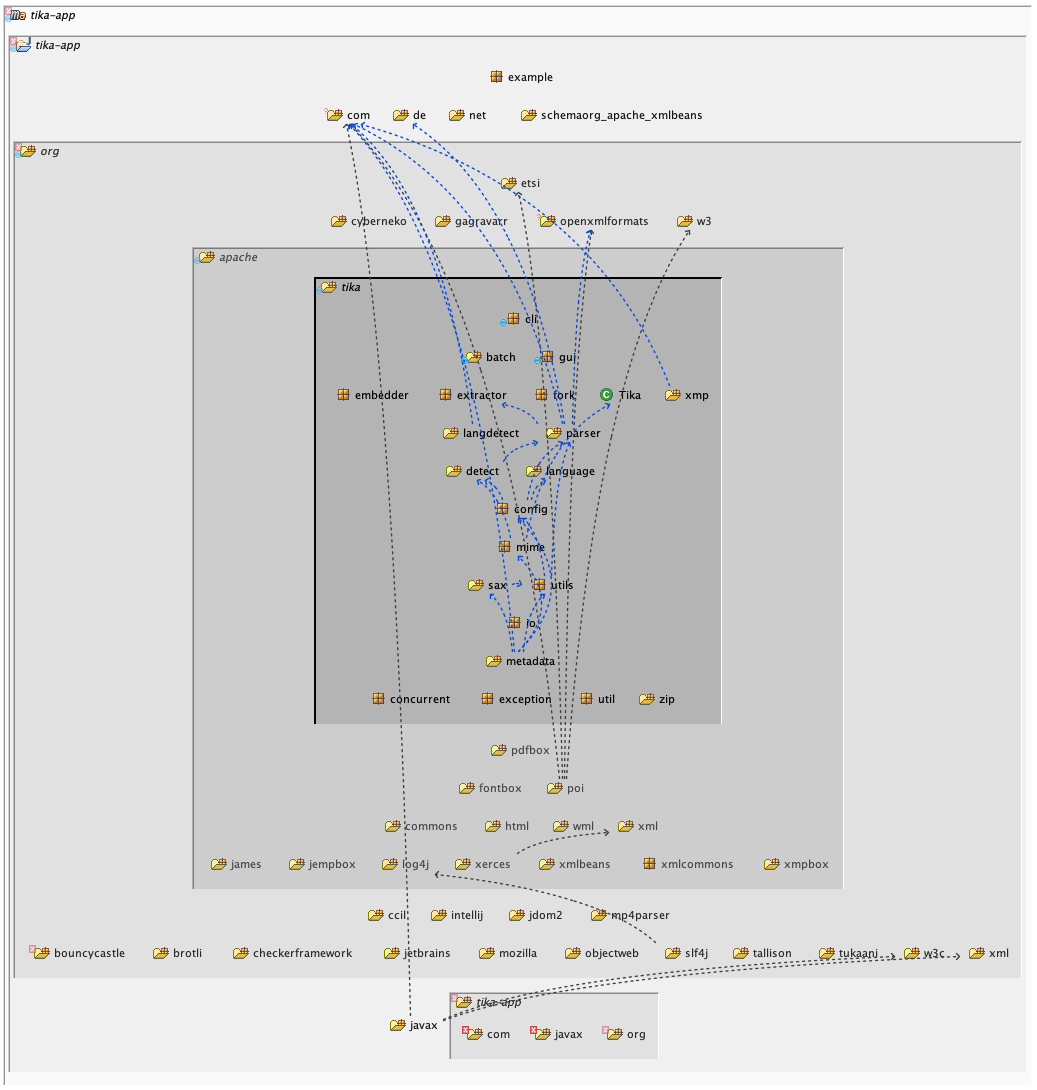
\includegraphics[width=\textwidth]{report/images/tika_app/s101.png}
    \caption{Structure101 overview of tika-app module.}
    \label{fig:tika_app/s101}
\end{figure}

\subsubsection{tika-core}
\begin{figure}[ht]
    \centering
    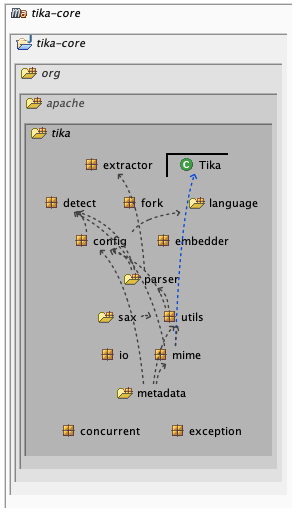
\includegraphics[width=0.5\textwidth]{report/images/tika_core/s101}
    \caption{Structure101 overview of tika-core module.}
    \label{fig:tika_core/s101}
\end{figure}

\end{document}
